I took this course in the Fall of 2024. That semester was a pretty low point for me mentally. Not
because of the course, but personal reasons. I was over school.


\section{Matrix Algebra and Systems of Linear Equations}
To understand what Matrix Algebra is, I have to make sure you understand what
a System of Linear Equations is. Thankfully, this is pretty straight forward.

\subsection{Systems of Linear Equations}
A system of Linear Equations is more than one Linear Equation

\begin{tcolorbox}[mybox]
    \textbf{Recall: } A \textit{Linear Equation} is an equation in the form
    \(a_1x_1 + \dots + a_{n} x_{n} +b = 0\), where \(x_1, \dots, x_{n}\) are the
    \textbf{variables} and \(b, a_1, \dots, a_n\) are the \textbf{coefficients}


    \vspace{1\baselineskip}

    If you forgot what a coefficient was, it's a number that doesn't change. e.g.
    \(\pi x^2 + 3x + 9\). \(\pi, 2\) and \(9\) are the coefficients.

    \vspace{1\baselineskip}

    And, you're killing me, if you forgot what a \textbf{variable} was: it's the
    number that DOES change. In the above example, the \(x\)'s are the variables.
\end{tcolorbox}


\begin{tcolorbox}[important]
     A linear equation can not have combined variables, for example:
    \begin{equation}
        3x_{1}x_{2} + x_{3} = 10
    \end{equation}
    is \textbf{invalid}
\end{tcolorbox}
So a system of Linear Equations is more than one of those, which we stack up into a matrix.
Boom, killed two birds with one stone there.

Consider the two equations \(2x^2 + 3x - 1 \) and \(9x^2 + x\), represented in matrix form
we have:
\begin{equation}
\begin{bmatrix}
    2x^2 + 3x - 1 \\
    9x^2 + x
\end{bmatrix}
\end{equation}

This leads to the next topic,
\subsection{Ways to represent Systems of Linear Equations}
Let's take the equation used in the above example. We can represent this in two ways:

\subsubsection{Coefficient Matrix}
The first way a \textbf{coefficients' matrix} is a matrix that is just the coefficients
of the problem, so we have:
\begin{equation}
    \begin{bmatrix}
        2 & 3 & -1 \\
        9 & 1 & 0
    \end{bmatrix}
\end{equation}

The -1 represents the \(-1x^0\) from the first equation and since there is none
in the second, it's replaced with \(0 x^0\)

\subsubsection{Adjacency Matrix}
Similarly, an Adjacency Matrix includes the solution, or \(b\). We use this more since
it's got some cool stuff going on and answers some important questions, but more on that
later. For right now, let's just show what it looks like:
\begin{equation}
    \begin{bmatrix}
        2 & 3 & -1 & b_1 \\
        9 & 1 & 0 & b_2
    \end{bmatrix}
\end{equation}


\subsubsection{now what?}

Okay, so now what? Well, first, maybe it's important to understand why we use
systems of linear equations and all of these fancy shmancy formats.

Say you have \$20.00 and you have to go out and buy some milk and a soda. You get to the store and
see that a gallon of milk is \$2.75 and a soda is \$2.50. You notice that the milk is on sale, so you want to see how many you can buy. Being the little math wizz you are, you come up with the equation
\begin{equation}
    \begin{split}
    2.75x + 2.50 &= 20.00 \\
    2.75x &= 17.25 \\
    x & \approx 6.27 \text{ gallons of milk}
    \end{split}
\end{equation}
but what happens if your Mom calls you and says OJ is on sale too, get as much as you can!
Well, now you have a problem, because you want to find the most amount of OJ (valued at \$1.25) and the most amount
of milk you can get with \$20.00. Insert Linear freakin' algebra.

You now have 2 equations you can put together.
\begin{equation}
    \begin{split}
        2.75x + 2.50 &= 20.00, \\
        2.75x + 1.25y &= 20.00.
    \end{split}
\end{equation}

You can try to solve this, and sure, it's not impossible, but what if I told you that
there was a much, much easier way to do this? Well, you have no choice, you can solve it yourself,
close and close this book, or you can see the better way.

\section{Row Reduction}
(Don't worry, we will solve the OJ problem (no, not whether the glove fit, Orange Juice)),


\section{Vector Spaces and Subspaces}
\subsection{Vector Spaces}
Vector Spaces are the areas (spaces) where vectors can "live", based on predefined parameters that can be \textit{added} and \textit{scaled} while satisfying 10 properties listed in the book (The important ones are listed.). If we think of a vector space say, H = \( \left\{ \begin{bmatrix} x \\ y \end{bmatrix}  : x \geq 0, y \geq 0 \right\} \in \mathbb{R}^2 \gets\) says \textit{A vector} \(x\) and \(y\) \textit{should be greater than 0 for both values, and would therefore fall in that vector space.} On a Cartesian plane (I swear, if you need to ask what this is), it would look something like this:
\begin{center} 
\includegraphics[width=200px]{8.3_vec_spaces.png} \end{center}
This then must satisfy 10 different properties (found in the text book, but I am only going to explain the 3 that we said to be the most useful. You can look up the other 7 if you have to.)
\begin{enumerate}
    \item The vector being tested must satisfy the \textbf{zero vector}.
    \item It must be \textbf{closed under addition} (In this example, it must be in \(\mathbb{R}^2\))
    \item It must be \textbf{closed under multiplication}. (Same thing, must be in \(\mathbb{R}^2\))
\end{enumerate}

\begin{tcolorbox}[mybox]
    In simplest terms, this just means that \(\vec{v} + \vec{w}\) and \(c\vec{w}\) must \textbf{stay in the set.}
\end{tcolorbox}

Now, lets do some actual math, shall we? Let us use the same example as above, \( \left\{ \begin{bmatrix} x \\ y \end{bmatrix}  : x \geq 0, y \geq 0 \right\} \in \mathbb{R}^2 \) and we have two vectors: \(\vec{w} = \begin{bmatrix} 2 \\ 1 \end{bmatrix}\) and \(\vec{u} = \begin{bmatrix} 1 \\ 1 \end{bmatrix}\).




\begin{center} 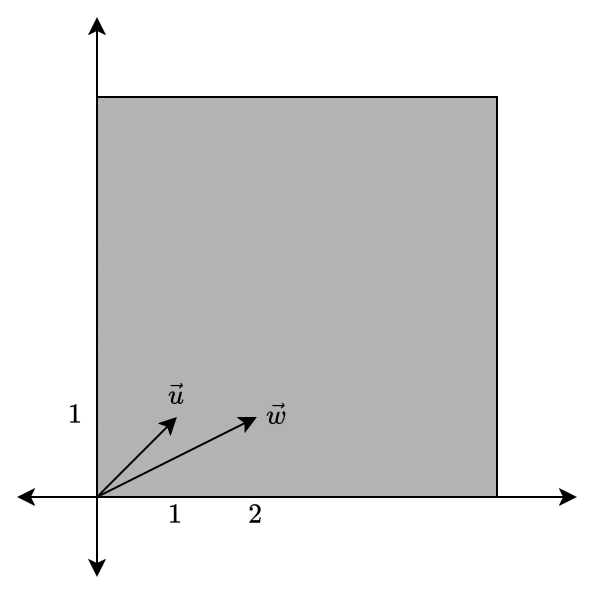
\includegraphics[width=200px]{8.3_vec_spaces_2.png} \end{center}
\subsection{Subspaces}
\textbf{Subspaces} are spaces in a \textit{vector space}. It's really just a more restricted area of the entire vector space that is being tested against. For example, when it says a vector that is in \(\mathbb{P}_n\), it's saying \textit{ a vector that is in the \textbf{BIGGER} set of } \(\mathbb{P}_n\)